%# -*- coding: utf-8-unix -*-
%%==================================================
%% chapter01.tex for SJTU Master Thesis
%%==================================================

%\bibliographystyle{sjtu2}%[此处用于每章都生产参考文献]

\chapter{绪论}
\label{chap:intro}



\section{研究背景及其意义}

过程控制系统(PCS, Process Control Systems),也称为工业控制系统(PCS,Industrial Control Systems),是一系列由监控和数据采集(SCADA)、可编程逻辑控制器(PLC)或分布式控制系统(DCS)等设备组成的工业生产过程的控制系统,并且可以收集和传输在制造过程期间获得的数据。 PCS可以是相对简单的系统,仅仅包含具有接收输入的传感器(通常称为主传感器),处理输入的控制器和处理输出的接收器。

PCS系统在全世界范围内不间断地监控和运行关键性的工业基础设施。PCS系统广泛应用并服务于电能产生和交付、石油天然气精炼和管道、水分配和处理、化学加工和生产、制药、食品饮料生产、铁路运输和空中交通管制以及离散制造[Stouffer11] [Weiss10] [Hentea08]。相比更贴近家庭的“智能电网”设备正在被集成到能量输送PCS系统中。这些新设备直接控制电表,允许电能流入我们的家庭并实时监测个人家庭的电能消耗。在医学上,PCS也运用于医院系统和常用的高科技医疗设备。

一方面,随着PCS系统越来越多的接入外部网络并且伴随着网络威胁的持续增加,PCS系统越来越容易受到能够破坏硬件的软件入侵的攻击,尤其是通用的计算和网络连接给关键基础设施带来全球恶意分子的电子攻击。控制系统已经被证明容易受到来自传统计算机病毒[1,2,3]、远程攻击[4]、内部攻击[5]和有针对性的策略攻击[6]的侵入。涉及的关键攻击目标主要包括核电和改进材料[3,6]、运输[7,4]、电力输送[8]、制造[1]、楼宇自动化[5]。
在一项对工业控制系统十年渗透测试结果的研究中,超过50%的报告表明控制系统的攻击已导致高于100万美元的损失[10]。在同一研究中还发现,41%的报告显示攻击可以导致“生产损失”,29%报告称网络攻击可以使PCS系统“丧失了查看或控制系统的能力”。在电力行业安全专家进行的调查中,发现能源供应商对他们自己的基础设施的安全性存在普遍的误解,例如他们认为控制系统与公共网络隔离,而且使用模糊的协议防止外部滥用的攻击[11]。此外安全研究人员还发现了针对控制系统的新型攻击。最近,研究人员发现智能电表中的漏洞允许窃取能量和拒绝供电[12,13],在电网的基本状态估计功能中发现的缺陷允许对整个传输和分配系统进行基于仪表的攻击[14]。

另一方面,从数据的角度来看,分布式PCS系统包括传感器数据采集,处理和控制命令。从现场传感器到端点功率控制网络设备(例如PLC)的信息路径实现了诸如状态估计和设备控制的工业系统应用。由于许多原因包括错误配置、传感器故障、通信故障或蓄意的虚假数据注入攻击都会影响甚至破坏信息路径内的数据完整性。实际上,PLC是在控制自动化目的的工业控制系统中广泛使用的多输入和多输出的微控制器设备。在系统的拓扑结构看来,噪声数据持续存在于系统中,但是由于用于检测和处理这样的数据的机制,才使得系统保持高水平的可靠性。然而最近的研究[20],[30]表明,恶意协调的虚假数据注入攻击可能能够绕过传统的检测噪声数据状态估计机制,所以这种攻击可能影响PCS系统状态估计应用程序进而操纵计算系统状态估计行为[18],[26],[28]。在系统的物理控制器看来,存在针对网络物理平台的控制器感知虚假数据注入攻击。该攻击需要关于变电站配置的有限本地高级信息,以及对向控制PLC设备反馈数据的变电站内的几个受感染传感器的控制。攻击考虑了由PLC运行的控制器算法,以通过操纵其输入值来生成恶意控制命令。值得注意的是,故障存在于系统各种控制单元中,故障检测和诊断机制则用于检测和处理控制系统中的故障问题使得各智能控制器能够以高可靠性的状态工作。然而本文构造了一种错误序列注入攻击能够避开检测故障机制,从而影响PCS系统中控制器的执行次序来操纵可编程控制器的逻辑行为,最终达到破坏受感染系统的目的。

过去十年中的受到的工业攻击表明,现实世界的控制系统及其组件缺乏实用的安全措施。

2007年,爱达荷国家实验室进行了极光攻击,以证明网络攻击如何破坏电网的物理组件[15]。攻击者获得了能够访问柴油发电机的控制网络,然后运行恶意计算机程序以快速打开和关闭发电机的断路器和电网的其余部分的相位参数,从而导致柴油发电机的爆炸。 

2008年,土耳其的一条管道遭到一个强大的爆炸袭击,在含水层以上的区域溢出了30000桶石油。此外,它花费英国石油每天500万美元的过境关税。攻击者通过利用无线摄像机通信软件的漏洞进入系统,然后深入到内部网络篡改了用于向控制室报告故障和泄漏的单元,并且控制阀站处的PLC以增加管道中的压力,从而导致爆炸。

2010年,Stuxnet计算机蠕虫感染在伊朗的14个工业现场的PLC,包括铀浓缩厂[4,17]。它通过受感染的USB闪存驱动器侵入到目标系统,然后Stuxnet通过感染可移动驱动器,在网络共享资源中复制本身并利用未修补的漏洞在网络中隐藏地传播,指示受感染的计算机连接到外部命令和控制服务器。最后中央服务器对PLC进行重新编程,以修改离心机的操作,以便由受损的PLC将它们分开[18]。 

在2015年,两个黑客展示了一个车辆的遥控器[19]。 零日漏洞使黑客无线控制车辆。车辆娱乐系统中的软件漏洞允许黑客对其进行远程控制,包括仪表板功能,转向,制动和传输,从而实现恶意动作,例如控制空调和音频,禁用发动机和制动器,以及控制车轮 [20]。据权威统计,截止2015年底,全球发生800余起针对工业控制系统的攻击事件,尤其是在最近几年存在越演越烈的趋势,具体如图\ref{pcsattack}所示。

\begin{figure}[!htp]
 \centering
 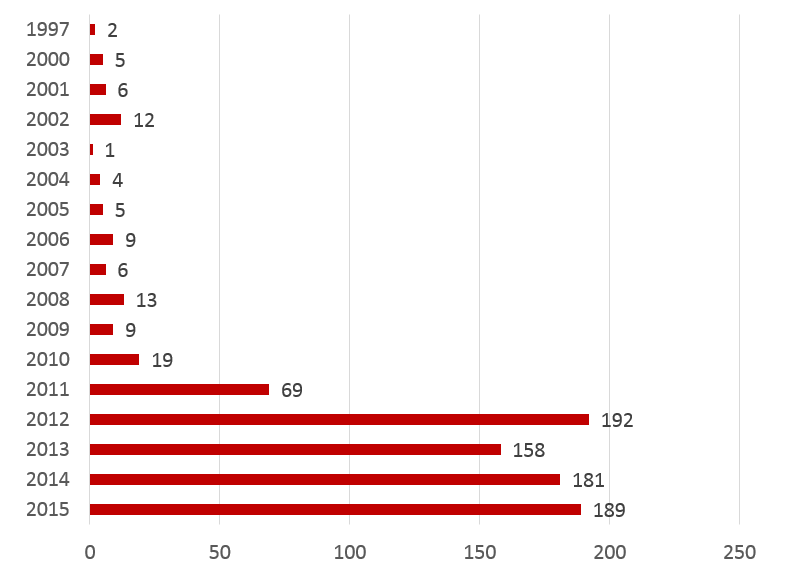
\includegraphics[width=14cm]{intro/PCSAttackEvent.png}
 \caption[fig:pcsattack]{1997-2015全球工业系统攻击事件.}
 \label{pcsattack}
\end{figure}


综上分析可以看出,不管是从网络信息安全还是从数据完整性的角度,PCS系统所面临的安全风险和入侵威胁都在不断增加,而且伴随着工业安全事故的数量逐年增加,相应带来的破坏和灾难也越发严重。所以,PCS系统的网络信息安全和数据安全已经成为越来越需要全面和深入研究的国家基础设施和关键领域。
正是在这种背景下,为了检测对PCS系统的入侵威胁,建立安全系统和关键国家基础设施安全的综合防御系统,本文重点谈久了基于PCS系统的入侵检测这样一个重要课题。

本文首先提出了对PLC的错误序列注入攻击,通过监视并控制PLC和实际物理设备之间的部分受感染传感器和足够的输出信号序列构造特定破坏序列注入到测量输入信号中。值得注意的是,在现有故障检测的条件下,我们利用容错率构造的攻击可以很好的绕开故障检测和诊断机制。根据控制系统不同层面的攻击特点,本文设计了一个双层检测和防御结构,以更好地保护SCADA系统。第一层主要是基于规范的程序攻击检测来应对网络侵入并攻击控制网络的情况,只有被检测并指示安全的程序和指令才能下载到可编程控制器设备中。基于第一层检测机制,我们可以保证运行在控制系统的程序的完备性和有效性,进而可以对控制器采集信号数据库,以执行第二层基于异常的数据完整性攻击检测。值得注意的是,我们创造性地提出了防御新型的控制器错误数据注入攻击尤其是错误序列注入攻击的检测和诊断方法,这是传统异常检测机制无法完成的工作。通过这两层检测,我们将为PCS系统构建一个完整的安全系统。

\section{过程控制系统与传统IT网络安全区别}


在过去,PCS使用专有硬件和软件,他们之间互连主要集中在总线通信。在20世纪90年代中期,人们将以太网和Microsoft Windows引入PCS,随后开发OPC接口,大大简化了本地与远程以及分布式通信问题,为此PCS也付出了暴露于以前仅为IT系统所知的安全威胁为代价。

此外,随着对工业系统的攻击在过去几年中迅速增加,企业的信息安全部门通常负责整个工厂的网络安全,包括其PCS。不幸的是,并不是所有的IT安全解决方案都适合PCS,因为PCS和IT系统之间存在根本的区别。此外,工业生产通常具有多个生产过程和PCS,并且一些工业生产过程自然比其他生产过程更关键。因此,在工厂中的各种PCS之间处理不同的安全性并不罕见。

虽然IT安全的良好剂量对工业控制系统安全至关重要,但是成功地保护控制系统需要额外的机制。工业控制系统的独特之处在于它需要将安全措施与大多数IT系统区分开来,其中一些因素包括控制系统放置在车间,而不是数据控制中心;它们存在置于危险环境或接近危险环境的风险;而且设备在平台上的平均寿命是在几十年而不是几年来衡量的也是不争的事实。

参考Belden工业以太网基础设施设计研讨会的信息,IT和PCS安全解决方案之间的差异有如下几个方面:
\begin{itemize}
	\item 性能要求
	\item 可靠性要求
	\item 操作系统和应用程序
	\item 风险管理目标
	\item 安全架构
	\item 安全目标
\end{itemize}

安全目标是两者之间的本质区别。例如,IT安全的第一目标集中于隐私,即保护数据;而PCS安全的第一目标是基于安全性,即保护该过程。

根据PCS本身特点,我们队其安全要求的问题又细分为三大类。这些问题是:

软目标:根据Belden,控制网络充满了所谓的“软”目标,即设备易受到网络接口干扰。许多工厂中的PC运行数周或数月,没有任何安全更新,有些甚至没有任何防病毒工具。此外,这些网络中的许多控制器是在网络安全不受关注的时代设计的,结果这些设备中的许多可能由于畸形的网络流量或甚至大量的正常流量而中断。

多路径:许多控制网络具有多种传输途径,网络安全威胁可以通过这些途径进入工厂。这些路径通常绕过工厂中的现有安全措施,有些甚至不出现在网络图上。例如,携带进出设施的笔记本电脑,或从一个PC移动到另一个PC的USB密钥。这些可以很容易地将恶意软件带入工厂,并迅速从一个系统传播到另一个系统。

平面网络:许多PCS网络仍然被实现为不相关子系统之间没有隔离的大且“平坦”网络。这意味着如果在设备中一部分出现问题,它可以非常快地传播到其他不相关的子系统,甚至到远程工厂站点。

根据参考文献[gervais12],对于PCS网络和IT网络的不同总结如下表\ref{intro:diffBetweenPCSandIT}
\newcommand{\tabincell}[2]{\begin{tabular}{@{}#1@{}}#2\end{tabular}}  
\begin{table}[!htp]
\centering
\caption{PCS与IT系统网络的区别}
\label{intro:diffBetweenPCSandIT}
\begin{tabular}{|p{2cm}|p{6cm}|p{6cm}|}
\hline
分类 & PCS系统 & IT系统 \\
\hline
优先级 & SRA(安全性,可靠性,可用性)是满足生产要求的最重要的特性。此外,发送到PLC的参数的完整性也是重要的。 & CIA(机密性,完整性,可用性)是IT中的优先考虑的安全因素。 \\
\hline
意识差异 & PCS工程师通常不能正确地解释恶意攻击者的能力。他们经常假设任何规范不允许的事情是不可能发生的。 & IT系统工程师认为如果攻击者能够获得对设备的物理访问,则很难保护它。 \\
\hline
风险管理 & 安全是主要关注的问题,即使安全问题可能会使安全受到威胁。 & 安全开始成为设计过程的组成部分。 \\
\hline
安全架构优先级 & 终端设备(如PLC)需要防止恶意攻击者。 & 数据资料需要保护。 \\
\hline
寿命 & 10-20年。 IT和PCS的融合可能会改变这个生命周期。 & 3-5年。 \\
\hline
实时要求 & 自动化设备具有严格的实时要求,因此需要满足最后期限。 & 通常没有严格的实时要求。 \\
\hline
物理交互 & 与设备,工作人员和生产过程的重要物理交互。 & 与环境的少量物理交互。 \\
\hline
资源约束 & 终端设备(PLC)具有有限的处理能力。 然而,近年来的设备的处理能力显着增加。 & IT系统通常具有重要和高效的处理能力。 \\
\hline
补丁管理 & 更新补丁很困难,因为可用性要求 需要开发定制解决方案。 & 补丁管理现在是一个标准过程。 静默更新在后台执行安装。 \\
\hline
供应商设备支持 & 通常需要原始供应商的支持。 & 支持来自各种来源的软件供应商。 \\
\hline
有限的物理访问组件 & 分布式系统使得对设备的访问困难且昂贵。 & 可以访问大多数IT系统。\\
\hline
\end{tabular}
\end{table}


\section{国内外研究现状}

\subsection{过程控制系统现存的攻击威胁}

传统过程控制系统受到的攻击计算机和网络威胁,例如内存侵入,目的是损害其一个或多个组件,以获得对系统行为的控制或者访问与进程相关的敏感数据。这里我们回顾近年来三类PCS漏洞的研究,第一类总体上研究PCS系统及其运营商的安全现状,第二类考虑PLC中的安全漏洞,第三类考虑传感器中的漏洞,在这种情况更侧重于智能电表,因为其是智能电网基础设施的重要组成部分。 

\begin{enumerate}
\item PCS总体安全现状:现有的研究[68]表明目前的PCS安全防护是有很大改进空间的。首先,因为PCS一直以来与因特网隔离并采用专有系统,所以经常被认为有很高安全性。然而,使用商用操作系统(例如,Microsoft Windows操作系统)和开放的标准网络协议使PCS不仅对于恶意攻击而且对因特网恶意软件的侵入感染都是开放的。例如,发生在俄亥俄州核发电站大面积破坏事件便是由于一些发电设施受到蠕虫病毒感染引起的。在10年内对100多个真实世界PCS进行渗透测试研究表明,在大多数情况下,这些PCS至少比标准补丁更新周期晚了一年。在某些情况下,将PCS与外部网络之间的DMZ隔离区域如果在几年内都没有更新的话,DoS攻击会变得很微弱。例如,在他们对网络连接的PLC的评估中,发现具有6字节分组的洪水攻击足以使PLC变得不可操作,导致所有状态丢失并迫使其重新启动。提高ICS安全性的另一个障碍是以下三个常见的错误[70]:
\begin{itemize}
\item 认为安全性可以通过隔离实现; 
\item 盲目部署安全技术提高安全性,例如防火墙、加密和防病毒软件的应用经常使系统操作者产生虚假的安全感;
\item 认为标准合规性可以保证系统安全,事实上即使北美能源可靠性公司提出的网络基础设施保护标准[71]也被批评为提供虚假的安全感[72]。 
\end{itemize}
\item 对PLC的攻击:PLC监视和操纵物理系统的状态,最常用的西门子PLC也被证明有漏洞。由于缺乏适当的会话饱满度,这些PLC使用的ISO-TSAP协议可以实现重放攻击[73],也可以绕过PLC认证上传有效载荷,并在PLC上执行任意命令。有研究表明用于监狱设施的西门子PLC也存在被操纵监狱门的可能性[74]。 
\item 对传感器的攻击:PCS的另一个关键组成单元是收集数据并将其传送回控制单元的传感器。智能电表作为演进智能电网的广泛部署的要素具有与传统模拟电表相同的形状因子[75]和多个增强特征:使用时间定价[76]、自动读表、电力质量监视和远程电源断开。现实世界智能计量系统的安全评估通常被认为是通过篡改测量值引发类似能源盗窃等一系列安全事故[77]。存在研究表明受测系统在被实施重放攻击时允许在在仪表的内存以及飞行中进行不可检测的篡改测量值操作。后续研究检查了来自多个供应商的计量表时发现允许针对任意仪表的DOS(拒绝服务)攻击的漏洞,而且可以对远程断开开关进行完全控制使得能够有目标地断开对客户的服务[78]。
\end{enumerate}

除了上述总结的传统安全威胁,这里我们着重考察PCS攻击的两个新方向。其中第一类构造了针对对手可能不具有完全访问权的PCS的程序篡改攻击。第二类攻击操纵传感器输入以误导控制系统尤其是可编程控制器执行动作。 
\begin{enumerate}
\item 程序篡改攻击:一种类型的攻击旨在收集有关受害者PCS的情报。例如,Duqu蠕虫病毒主要收集关于受害者系统的信息[79],然后将其转发到命令和控制服务器。对PCS的另一种类型的攻击旨在影响受害者系统的物理行为,这种攻击的最着名的例子是Stuxnet蠕虫,其攻击手段主要是操纵用于铀浓缩的一组离心机的参数。这样的攻击有两个阶段:感染和上传恶意程序。传统来说一旦攻击者破坏了信息系统,上传预先构建的恶意程序是不难的。这是因为攻击者通常有一个被攻击的软件的副本。然而对于PCS则不一定是这种情况,根据攻击者实施的攻击类型,恶意程序的构造可能容易出错或几乎不可能。恶意程序是无区别的或有针对性的,不加区分的恶意程序执行随机攻击,在受害者PCS的机制内引起恶意行为。有几种方式恶意软件可以在获得对一个或多个受害者PCS PLC的访问时自动构造不加区分的有效载荷[80]。这里的假设是,如果恶意软件能够写入PLC代码区域,则它还必须能够从PLC代码区域进行读取。由于具有读取PLC代码的能力,首先恶意软件推断出被称为互锁的基本安全属性[82],并生成一个恶意程序,其可以违反尽可能多的安全属性。 其次恶意软件识别系统中的主定时环路。考虑交通灯的示例,其中主循环确保每种颜色的光在特定时间段内依次有效。然后,恶意软件可以构造违反定时循环的恶意程序,例如通过允许某些光重叠。 最后在总线枚举技术中,恶意软件使用标准化标识符(如现场总线ID)来找到受害系统中的特定设备[83]。
\item 错误数据注入(FDI)攻击:在FDI攻击中,攻击者选择一组注入到一个或多个控制器的传感器,然后向这些传感器提供精心制作的恶意值,从而使控制器获得预期的结果。例如,如果所提供的恶意值告诉控制器温度变得太低,则它将令加热元件不断增加温度,即使实际温度很好也会导致未检测到的设备过热。最早的FDI攻击目标是电力系统状态估计[85]。状态估计是分布式控制系统中的重要步骤,其中基于多个可观测量来估计实际物理状态。电力系统状态估计确定电力负载如何分布在输电网络中的各种高压线路和变电站上。人为干扰相量测量单元(PMU)的子集可导致不正确的状态估计。[86]报道了基于卡尔曼滤波的状态估计的FDI攻击。卡尔曼滤波器是比线性和直流系统模型更一般的状态估计形式,基于卡尔曼滤波器的状态估计器对FDI攻击的敏感性取决于设计系统的固有属性[86]。如果基础状态转移矩阵包含不稳定的特征值,则系统只保证通过FDI攻击是可控的。这不仅对攻击具有重要的意义,而且对于针对FDI攻击的防御具有重要的意义,因为缺乏不稳定特征值的系统可能不会被完全攻击。

\end{enumerate}




\subsection{}

\section{论文组织结构}

